%%%%%%%%%%%%%%%%%%%%%%%%%%%%%%%%%%%%%%%%%%%%%%%%%%%%%%%%%%%%%%%%%%%%%%%%%%%%%%%%
% test.tex
%%%%%%%%%%%%%%%%%%%%%%%%%%%%%%%%%%%%%%%%%%%%%%%%%%%%%%%%%%%%%%%%%%%%%%%%%%%%%%%%
%
% Authors:
% - Sébastien Julliot
%
% Contributors:
% - Unknown for now
%
%%%%%%%%%%%%%%%%%%%%%%%%%%%%%%%%%%%%%%%%%%%%%%%%%%%%%%%%%%%%%%%%%%%%%%%%%%%%%%%%


\documentclass{42}

\usepackage{amsmath, amsfonts, amssymb}


%%%%%%%%%%%%%%%%%%%%%%%%%%%%%%%%%%%%%%%%%%%%%%%%%%%%%%%%%%%%%%%%%%%%%%%%%%%%%%%%
% Prologue
%%%%%%%%%%%%%%%%%%%%%%%%%%%%%%%%%%%%%%%%%%%%%%%%%%%%%%%%%%%%%%%%%%%%%%%%%%%%%%%%

\begin{document}

%Table des matieres
\title{Computor v1}
\subtitle{}

\member {42 staff}{staff@42.fr}

\summary
{

Ce projet est le premier d'une série ayant pour but de vous faire renouer avec les maths, qui vous seront très utiles -voire nécessaires- pour de nombreux autres projets.
}

\maketitle

\tableofcontents

% Valeurs utilisees pour la generation de headers d'exercices
\turnindir{svn+ssh://rendus@rendus.42.fr/sujetdetest-2142-login\_x}


\graphicspath{{images/}}

\newpage
%%%%%%%%%%%%%%%%%%%%%%%%%%%%%%%%%%%%%%%%%%%%%%%%%%%%%%%%%%%%%%%%%%%%%%%%%%%%%%%%
% Start document
%%%%%%%%%%%%%%%%%%%%%%%%%%%%%%%%%%%%%%%%%%%%%%%%%%%%%%%%%%%%%%%%%%%%%%%%%%%%%%%%

\chapter{Préambule}
\section{Version 1}

\hint
{
	La version 2 a raison.
}

\begin{flushleft}
Un polynôme est une expression formelle de la forme:
	\begin{equation}
	P(X)=\sum_{k=0}^{n} a_k X^k
	\end{equation}
	où X est appelé indéterminée du polynôme.
	\newline
	\newline
	Le produit de deux polynômes est ainsi défini par
	\begin{equation}
	\left(\sum_{i=0}^n a_iX^i\right)\left(\sum_{j=0}^m b_jX^j\right) = \sum_{k=0}^{n+m} \left(\sum_{i+j = k}a_ib_j\right)X^k.
	\end{equation}
\end{flushleft}
\begin{center}
	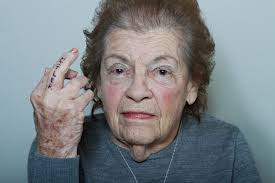
\includegraphics[scale=0.35]{what1}
	
\includegraphics[scale=0.35]{what2}
	
\includegraphics[scale=0.35]{what3}
	
\includegraphics[scale=0.35]{what4}
	
\includegraphics[scale=0.35]{what5}
	
\includegraphics[scale=0.35]{what6}
	
\includegraphics[scale=0.35]{what7}
	
\includegraphics[scale=0.35]{what8}
\end{center}

\newpage
\section{Version 2}

\subsection{Approche intuitive}

\hint
{
	La version 1 se trompe.
}
\begin{flushleft}
Essayons maintenant d'en donner une approche plus compréhensible, et de justifier l'existence de ce sujet.

~\\
Si je vous dis que pour me prendre un thé (tout mathématicien qui se respecte boit du thé et non du café, question de principe), je:
\newline
\begin{itemize}
	\item Descends trois étages.
	\item Traverse le couloir en direction des machines.
\end{itemize}
~\\
Et que je vous demande comment rejoindre mon poste, vous me direz que je dois:
\newline
\begin{itemize}
	\item Traverser le couloir dans l'autre sens.
	\item Remonter trois étages.
\end{itemize}
~\\
~\\
De même, si je vous dis que pour aller de chez moi à 42 je:
\newline
\begin{itemize}
	\item Vais au métro.
	\item Prends la 14 de Olympiades à Saint-Lazare.
	\item Prends la 13 de Saint-Lazare à Porte de Clichy.
	\item Vais jusqu'à 42.
\end{itemize}
~\\
Vous me direz que pour rentrer, je dois:
\newline
\begin{itemize}
	\item Aller jusqu'au métro.
	\item Prendre la 13 jusqu'à Saint-Lazare.
	\item Changer pour prendre la 14 jusqu'à Olympiades.
	\item Aller jusqu'à ma porte.
\end{itemize}

~\\
~\\
Si vous avez compris ça, vous avez tout compris.
\end{flushleft}

\newpage

\subsection{Lien avec les mathématiques}

\begin{flushleft}
Dans un calcul on effectue, dans l'ordre:
\newline
\begin{itemize}
	\item Les calculs dans les parenthèses
	\item Les multiplications
	\item Les additions
\end{itemize}
~\\
Cela signifie que si $x = 4$ et que vous avez à calculer $3 * (x - 5) + 12$ alors
\begin{align}
	3 * (x - 5) + 12	&= 3 * (4 {\color{red} - } 5) + 12 \\
					&= 3 {\color{red} * } (-1) + 12 \\
					&= -3 {\color{red}+} 12 \\
					&= 9
\end{align}
\end{flushleft}
~\\
\begin{center}
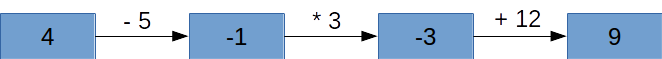
\includegraphics[scale=0.8]{illustration_resolution_equation.png}
\end{center}
Ici, on est partis de x pour arriver au résultat. Résoudre une équation, c'est simplement faire le chemin en sens inverse. \newline \newline
Donc, pour résoudre $3 * (x - 5) + 12 = 18$, on fait (en partant de la droite):
\begin{center}
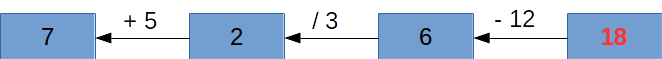
\includegraphics[scale=0.8]{illustration_resolution_equation_rev.png}
\end{center}
Et la solution de cette équation est bien 7. $\backslash$o/
\hint
{
	Dans le cas d'une équation de degré 2, commencez par la mettre sous forme canonique.
}

\info
{
Voici une liste non exhaustive des sujets où savoir ce que sont et comment manipuler les polinômes pourrait bien vous être utile:
	\begin{itemize}
	\item Fractol
	\item RT
	\item mod1
	\item Expert System
	\item Infin Mult
\end{itemize}

Par ailleurs, ce petit sujet sera complété par d'autres dont le but est de vous offrir d'aborder plus sereinement les sujets faisant intervenir des mathématiques, tout en comprenant ce que vous faites.
}
\chapter{Partie obligatoire}

\extitle{Computor v1}
\exfiles{A votre convenance}

\makeheaderbasic

Le but de l'exercice est d'écrire un programme qui résout des équations polynomiales.

Exemples:

\begin{42console}
Entrez une equation: 5 * X^0 + 4 * X^1 - 9.3 * X^2 = 1 * X^0
Sous forme reduite : 4 * X^0 + 4 * X^1 - 9.3 * X^2 = 0
Cette equation est de degre 2.
Son discriminant est strictement positif, elle a donc exactement deux solutions reelles :
0.905239
-0.475131
\end{42console}

\begin{42console}
Entrez une equation: 5 * X^0 + 4 * X^1 = 4 * X^0
Sous forme reduite : 1 * X^0 + 4 * X^1 = 0
Cette equation est de degre 1 et a pour solution -0.25.
\end{42console}

\begin{42console}
Entrez une equation: 8 * X^0 - 6 * X^1 + 0 * X^2 - 5.6 * X^3 = 3 * X^0
Sous forme reduite : 5 * X^0 - 6 * X^1 + 0 * X^2 - 5.6 * X^3 = 0
L'equation est de degre superieur a 2, on ne sait pas resoudre.
\end{42console}

NB: Pour la partie obligatoire, on considèrera l'entrée bien formatée (ie. tous les termes sont de la forme \begin{equation}coefficient * X^{puissance}\end{equation}. Les puissances sont bien ordonnées et toutes présentes.

\info
{
	La résolution des équations de degré trois ou plus n'est pas demandée, et sera envisagée ultérieurement.
}

\newpage

\chapter{Partie bonus}

Voici une liste de bonus qu'il pourrait être utile d'implémenter:



\begin{itemize}
	\item Gérer les erreurs sur l'entrée
	\item Gérer les entrées sorties sous forme naturelle
\begin{42console}
Entrez une equation: 5 + 4 * X + X^2= X^2
Sous forme reduite : 5 + 4 * X = 0
Cette equation est de degre 1 et a pour solution -1.25.
\end{42console}
	\item Afficher la (les) solution sous forme de fraction irréductible quand c'est intéressant
	\item Afficher des étapes intermédiaires
	\item ...
\end{itemize}

\chapter{Consignes}
\begin{flushleft}
	\begin{itemize}
		\item Pensez aux solutions complexes quand le degré vaut 2 ;)
		\item Le choix du langage est à votre discrétion.

		\item Cela dit, vous n'avez évidemment droit à aucune fonction mathématique (hors addition et multiplication de réels) que vous n'ayez pas implémentée vous-mêmes.

		\item Si vous travaillez en C, vous rendrez un Makefile contenant les règles habituelles et respecterez bien sûr la norme.
	\end{itemize}
\end{flushleft}
Bon courage !

%%%%%%%%%%%%%%%%%%%%%%%%%%%%%%%%%%%%%%%%%%%%%%%%%%%%%%%%%%%%%%%%%%%%%%%%%%%%%%%%
% End document
%%%%%%%%%%%%%%%%%%%%%%%%%%%%%%%%%%%%%%%%%%%%%%%%%%%%%%%%%%%%%%%%%%%%%%%%%%%%%%%%
\end{document}
